\section{Parallel Tractability of Ontology Materialization in OWL}
\label{sec:ptonto}

In this section, we study the issue of parallel tractability
for materialization of DL-Lite and DHL (DHL($\circ$)) ontologies
based on Algorithm~$\mathsf{A}_{\text{opt}}$. We show that, for any class $\mathbb{O}$ of
DL-Lite$_{\text{core}}$ or DL-Lite$_\mathcal{R}$ ontologies,
there exists a poly-logarithmically bounded function $\psi$
such that Algorithm~$\mathsf{A}_{\text{opt}}^{\psi}$ can handle materialization of the ontologies in $\mathbb{O}$.
However, for DHL and DHL($\circ$), there exist ontology classes such that Algorithm~$\mathsf{A}_{\text{opt}}^\psi$
does not work. We illustrate the reason why Algorithm~$\mathsf{A}_{\text{opt}}^\psi$ cannot always
work by studying specific cases.
Further, we propose to restrict the usage of DHL and DHL($\circ$) in order to achieve parallel tractability
of materialization.

\subsection{Materialization of DL-Lite Ontologies via Algorithm~$\mathsf{A}_{\text{opt}}$}

In this part, we show how to use Algorithm~$\mathsf{A}_{\text{opt}}$ to handle
DL-Lite materialization and analyze its parallel tractability.
Based on the analysis, we have that, for any DL-Lite$_{\text{core}}$ or DL-Lite$_\mathcal{R}$ ontology
there always exists an SWD path for each atom of the form $A(a)$ or $R(a,b)$.
In other words, all atoms of the forms $A(a)$ and $R(a,b)$ can be added to
the constructed materialization graph in the first iteration of \ref{alg3:updateG}
by performing Algorithm~$\mathsf{A}_{\text{opt}}$.

In order to show how Algorithm~$\mathsf{A}_{\text{opt}}$ handles DL-Lite materialization,
we use the following example.

\begin{example}\label{exp:dllite}
Given a DL-Lite ontology $\mathcal{O}_{\text{ex}_5}$
where the TBox and RBox contain the following axioms:
$A\sqsubseteq B_1$, $A\sqsubseteq B_2$, $B_1\sqcap B_2\sqsubseteq\bot$,
$\exists R.B_2\sqsubseteq\bot$, $Q\sqsubseteq S^-$, $S\sqsubseteq R$;
its ABox contains an assertion $Q(a,b)$.
We denote the corresponding datalog program of $\mathcal{O}_{\text{ex}_5}$ by $P_{\text{ex}_5}=\langle R, \textbf{I}\rangle$,
where $R$ contains the rules that are transformed from the above axioms; $\textbf{I}$ contains $Q(a,b)$
as the only fact.
The unique materialization graph of $P_{\text{ex}_5}$ is denoted by $\mathcal{G}_{\text{ex}_5}$ (see Figure~\ref{fig:ex2}).
\end{example}

\begin{figure}[htbp]
\begin{center}
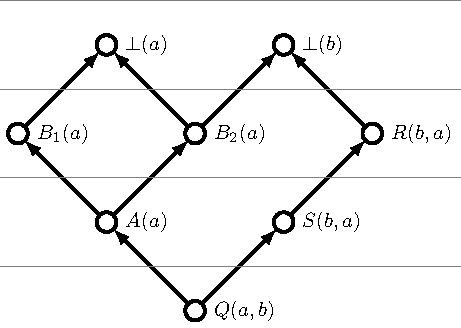
\includegraphics[width=0.5\textwidth]{fig-dllite.pdf}
\caption{The materialization graph of $\mathcal{O}_{\text{ex}_5}$}
\label{fig:ex2}
\end{center}
\end{figure}

Consider performing Algorithm~$\mathsf{A}_{\text{opt}}$ on the ontology $\mathcal{O}_{\text{ex}_5}$ in Example~\ref{exp:dllite}.
(\uppercase\expandafter{\romannumeral1}) First, Algorithm~$\mathsf{A}_{\text{opt}}$ adds all ABox assertions (only $Q(a,b)$ here)
to the initially empty graph $\mathcal{G}_{\text{ex}_5}$ (\ref{alg3:addFacts} of Algorithm~$\mathsf{A}_{\text{opt}}$).
(\uppercase\expandafter{\romannumeral2}) In the first iteration of
\ref{alg3:updateG}, Algorithm~$\mathsf{A}_{\text{opt}}$ checks that all of the nodes
$A(a)$, $S(b,a)$, $B_1(a)$, $B_2(a)$ and $R(b,a)$ have corresponding SWD paths
starting from $Q(a,b)$. Thus, Algorithm~$\mathsf{A}_{\text{opt}}$
adds these nodes to $\mathcal{G}_{\text{ex}_5}$ immediately. We take an example of node $B_1(a)$,
for which an SWD path $(Q(a,b),A(a),B_1(a))$ exists.
When updating $\mathcal{G}_{\text{ex}_5}$ by adding $B_1(a)$ to it,
Algorithm~$\mathsf{A}_{\text{opt}}$ first checks whether the parent node $A(a)$ of $B_1(a)$
has been in $\mathcal{G}_{\text{ex}_5}$; if $A(a)$ is already in $\mathcal{G}_{\text{ex}_5}$, $B_1(a)$
is added to $\mathcal{G}_{\text{ex}_5}$ by creating an edge pointing from $A(a)$ to $B_1(a)$;
if $A(a)$ has not been added to $\mathcal{G}_{\text{ex}_5}$,
Algorithm~$\mathsf{A}_{\text{opt}}$ adds $A(a)$ ($B_1(a)$, respectively)
to $\mathcal{G}_{\text{ex}_5}$ and creates an edge pointing from
$Q(a,b)$ to $A(a)$ (an edge pointing from $A(a)$ to $B_1(a)$, respectively).\footnote{These two cases may happen simultaneously,
since node $A(a)$ and node $B_1(a)$ are being processed in parallel.} The other nodes
$A(a)$, $S(b,a)$, $B_2(a)$ and $R(b,a)$ are processed similarly.
(\uppercase\expandafter{\romannumeral3})
The two nodes $\bot(a)$ and $\bot(b)$
have no SWD path in the first iteration of \ref{alg3:updateG}.
They are left to be processed in the second iteration.
(\uppercase\expandafter{\romannumeral4})
Finally, Algorithm~$\mathsf{A}_{\text{opt}}$ finishes constructing $\mathcal{G}_{\text{ex}_5}$
after two iterations (\ref{alg3:halt}).

From the above example, we can observe that SWD paths exist
for all nodes except $\bot(a)$ and $\bot(b)$ in the first iteration of Algorithm~$\mathsf{A}_{\text{opt}}$.
Further, we give the following lemma that holds for any DL-Lite$_{\text{core}}$ or DL-Lite$_\mathcal{R}$ ontology.

\begin{lemma}\label{lemma:dllite}
For any DL-Lite$_{\text{core}}$ or DL-Lite$_\mathcal{R}$ ontology $\mathcal{O}$, there exists a materialization graph $\mathcal{G}$ such that
each atom of the form $A(x)$ ($A\neq\bot$) or $R(x,y)$ in $\mathcal{G}$ has an SWD path.
\end{lemma}

The above lemma guarantees that all atoms of the form $A(x)$ ($A\neq\bot$) or $R(x,y)$
have to be added to the constructed materialization graph in the first iteration of
\ref{alg3:updateG} by applying Algorithm~$\mathsf{A}_{\text{opt}}$.
For each atom of the form $\bot(x)$, there may not exist an SWD path in the first iteration
of \ref{alg3:updateG}, since its derivability depends on its two parent nodes
(see nodes $\bot(a)$ and $\bot(b)$ in $\mathcal{G}_{\text{ex}_5}$ of
Example~\ref{exp:dllite}). On the other hand, according to the syntax of DL-Lite,
$\bot$ does not occur on the left-hand side of any axiom. In other words,
an atom of the form $\bot(x)$ cannot be the parent of any other node.
This allows for adding all atoms of the form $\bot(x)$ to the constructed materialization graph in at most two iterations of
\ref{alg3:updateG} by applying Algorithm~$\mathsf{A}_{\text{opt}}$.
Based on the above discussion, for any DL-Lite ontology $\mathcal{O}$,
there always exists a poly-logarithmically bounded function $\psi$ such that
Algorithm~$\mathsf{A}_{\text{opt}}^{\psi}$ can handle the materialization of $\mathcal{O}$;
more precisely, we can set that $\psi=2$. This result is consistent with
that by \citet{CalvaneseGLLR07}.
Formally, we use $\mathcal{D}_{\textit{dl\_lite}}$
to denote the set of all DL-Lite$_{\text{core}}$ and DL-Lite$_\mathcal{R}$ ontologies and give the following theorem.

\begin{theorem}\label{theorem:dl-lite}
There exists a poly-logarithmically bounded function $\psi$ such that
$\mathcal{D}_{\textit{dl\_lite}}\subseteq\mathcal{D}_{\mathsf{A}_{\text{opt}}^{\psi}}$.
\end{theorem}


\subsection{Parallel Tractability of  DHL Materialization}
\label{sec:DHL}

In this part, we study whether Algorithm~$\mathsf{A}_{\text{opt}}^\psi$ can handle DHL ontologies.
Unfortunately there exist DHL ontology classes such that Algorithm~$\mathsf{A}_{\text{opt}}^\psi$
does not work for any poly-lo\-ga\-rith\-mi\-cal\-ly bounded function $\psi$.
In the following, we first give such a case
to illustrate the reason why Algorithm~$\mathsf{A}_{\text{opt}}^\psi$ cannot work.
Based on the analysis of this case, we propose to restrict
the usage of DHL in order to achieve parallel tractability
of materialization.

We find that, an unlimited usage of axioms of the
form $B_1\sqcap B_2\sqsubseteq A$
makes it impossible for Algorithm~$\mathsf{A}_{\text{opt}}$ to construct a materialization graph
in a poly-logarithmic number of iterations of \ref{alg3:updateG}.
We use the following example to illustrate this.

\begin{figure}[htbp]
\begin{center}
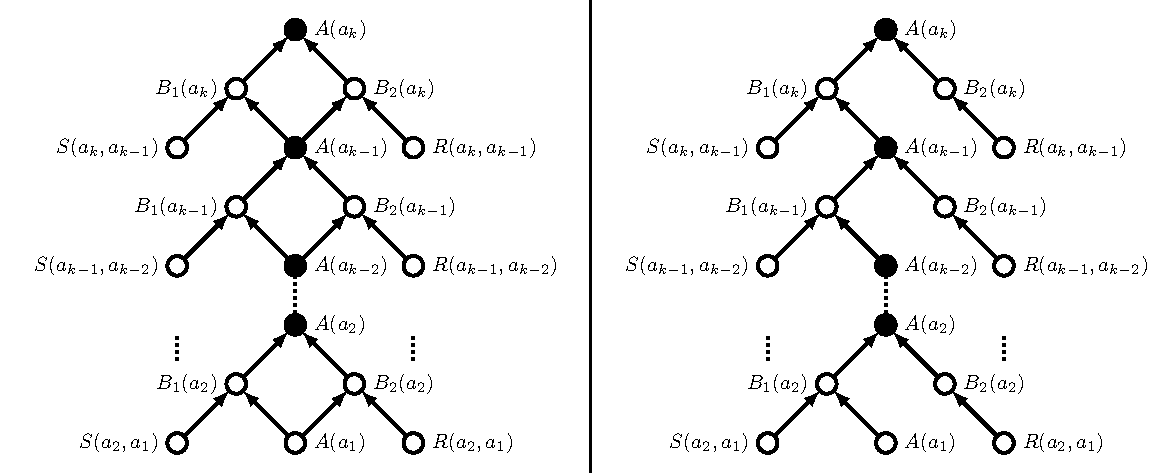
\includegraphics[width=\textwidth]{fig-pathtwist.pdf}
\caption{The materialization graph of $\mathcal{O}_{\text{ex}_6}$
  (left) and of $\mathcal{O}_{\text{ex}_7}$ (right)}
\label{fig:ex3_4}
\end{center}
\end{figure}

\begin{example}\label{exp:dhl}
Given a DHL ontology $\mathcal{O}_{\text{ex}_6}$ where the TBox contains three axioms:
$B_1\sqcap B_2\sqsubseteq A$, $\exists S.A\sqsubseteq B_1$ and $\exists R.A\sqsubseteq B_2$;
the ABox is $\{S(a_i,a_{i-1}), R(a_i,a_{i-1}), A(a_1)\}$
for $2\leq i\leq k$ and $k$ an integer greater than $2$.
We denote the corresponding datalog program of $\mathcal{O}_{\text{ex}_6}$ by $P_{\text{ex}_6}=\langle R, \textbf{I}\rangle$,
where $R$ contains three rules: `$B_1(x),B_2(x)\rightarrow A(x)$',`$S(x,y),A(y)\rightarrow B_1(x)$' and `$R(x,y),A(y)\rightarrow B_2(x)$'.
The materialization graph of $P_{\text{ex}_6}$ constructed by
$\mathsf{A}_{\text{opt}}$ is denoted by $\mathcal{G}_{\text{ex}_6}$
(see Figure~\ref{fig:ex3_4}~(left)).
\end{example}

One can check that $\mathcal{G}_{\text{ex}_6}$ is the unique materialization graph of $P_{\text{ex}_6}$.
Observe that there exists a path (e.g., $A(a_1),B_1(a_2),A(a_2),\ldots,A(a_k)$) between $A(a_1)$ and $A(a_k)$.
When performing Algorithm~$\mathsf{A}_{\text{opt}}$ on $P_{\text{ex}_6}$, it can be checked that
each node of the form $A(a_i)$ (filled with black color,
and $2\leq i\leq k$) has no SWD path until the $i^{th}$ iteration;
in the $i^{th}$ iteration, the parent nodes of $A(a_i)$ have been added to $\mathcal{G}_{\text{ex}_6}$,
and, $A(a_i)$ can also be added to $\mathcal{G}_{\text{ex}_6}$.
Similar to the datalog program class $\mathbb{P}_{\text{ex}_1}$, we can also get a
datalog program class $\mathbb{P}_{\text{ex}_6}$ for the ontology $\mathcal{O}_{\text{ex}_6}$
when $k$ is a variable. Based on the above analysis, Algorithm~$\mathsf{A}_{\text{opt}}$ cannot complete the materialization
for the datalog programs of $\mathbb{P}_{\text{ex}_6}$ in a poly-logarithmic
number of iterations.
The intuitive reason is that at least two paths exist
from $A(a_1)$ to $A(a_k)$. These paths \emph{twist} mutually and share the same joint nodes (see the black nodes).
This invalidates the optimization used in Algorithm~$\mathsf{A}_{\text{opt}}$.
That is, for each node $A(a_i)$, $2\leq i\leq k$, until its parents ($B_1(a_i)$ and $B_2(a_i)$) are added
to $\mathcal{G}_{\text{ex}_6}$, there would not exist an available SWD path for $A(a_i)$.
We use the term `\emph{path twisting}' to refer to such cases.

In order to make Algorithm~$\mathsf{A}_{\text{opt}}$ terminate in a poly-logarithmic number of iterations,
we consider restricting the usage of axioms of the form $B_1\sqcap B_2\sqsubseteq A$
to avoid `path twisting'. An intuitive idea is to
ensure that \emph{there is only one path between each two atoms of the form $A(x)$
generated from the rules corresponding to (T1)}.
We explain it by using the following example where the ontology is modified from
that in Example~\ref{exp:dhl}.

\begin{example}\label{exp:simpleC}
Consider an ontology $\mathcal{O}_{\text{ex}_7}$ where the TBox contains three axioms:
$B_1\sqcap B_2\sqsubseteq A$, $\exists S.A\sqsubseteq B_1$ and $B_3\sqsubseteq B_2$;
the ABox is $\{S(a_i,a_{i-1}), B_3(a_i), A(a_1)\}$
for $2\leq i\leq k$ and $k$ an integer greater than $2$.
We denote the corresponding datalog program by $P_{\text{ex}_7}$ where the rule set contains:
`$B_1(x),B_2(x)\rightarrow A(x)$',`$S(x,y),A(y)\rightarrow B_1(x)$' and `$B_3(x)\rightarrow B_2(x)$'.
$P_{\text{ex}_7}$ has a unique materialization graph denoted by $\mathcal{G}_{\text{ex}_7}$ (see Figure~\ref{fig:ex3_4}~(right)).
\end{example}

In the above example, for the axiom $B_1\sqcap B_2\sqsubseteq A$, all derived atoms
of the form $B_2(x)$ must not be child nodes of an atom $A(y)$ for some $y$.
This ensures that only one path exists between each two nodes among $A(a_2),\ldots,A(a_k)$.
Further, when constructing $\mathcal{G}_{\text{ex}_7}$, Algorithm~$\mathsf{A}_{\text{opt}}$ can terminate after
two iterations of \ref{alg3:updateG}. Specifically, in the first iteration, Algorithm~$\mathsf{A}_{\text{opt}}$
adds all of the nodes $B_3(a_i)$ and $B_2(a_i)$, $2\leq i\leq k$, to $\mathcal{G}_{\text{ex}_7}$
since they have corresponding SWD paths;
after that, all other nodes
can be added to $\mathcal{G}_{\text{ex}_7}$ in the second iteration (because each
node has an SWD path).
Motivated by this example, we consider restricting the usage of
the axioms $B_1\sqcap B_2\sqsubseteq A$
such that all atoms of the form $B_1(x)$ or $B_2(x)$ cannot be generated by an atom $A(y)$
for some $y$.
To this end, we first define \emph{simple concepts} as follows:

\begin{definition}
Given an ontology $\mathcal{O}=\langle\mathcal{T},\mathcal{R},\mathcal{A}\rangle$,
a concept $A\in\textbf{CN}$ is simple, if (1) $A$ does not occur on the right-hand side
of some axiom; or (2) $A$ satisfies the following conditions:
\begin{enumerate}[leftmargin=4ex,label=\arabic*.]
\item for each $B\sqsubseteq A\in\mathcal{T}$, $B$ is simple;
\item for each $\exists R.B\sqsubseteq A\in\mathcal{T}$, $B$ is simple;
\item there is no axiom of the form $B_1\sqcap B_2\sqsubseteq A$ in $\mathcal{T}$.
\end{enumerate}
\end{definition}

Based on simple concepts, we restrict DHL ontologies such that, in all axioms of the
form $B_1\sqcap B_2\sqsubseteq A$, at least one concept of $B_1$ and $B_2$ should be a simple concept
(we call this the \emph{simple-concept restriction}).
Intuitively, for such restricted DHL ontologies, the situation of `path twisting' does not happen.
This is because, for each axiom of the form $B_1\sqcap B_2\sqsubseteq
A$ such that, w.l.o.g., $B_1$
is a simple concept, none of the ancestors of $B_1(x)$ for some $x$
is generated from the rules corresponding to (T1).

\begin{example}
In the ontology of Example~\ref{exp:dhl}, all of $A$, $B_1$ and $B_2$ are
non-simple concepts.
In the ontology of Example~\ref{exp:simpleC}, $A$ and $B_1$ are non-simple concepts,
while $B_3$ and $B_2$ are simple concepts. Further, it can be checked that
the ontology  of Example~\ref{exp:simpleC} follows the simple-concept restriction
and can be handled by Algorithm~$\mathsf{A}_{\text{opt}}^\psi$ for some poly-logarithmic function $\psi$.
\end{example}

We define the following class of DHL ontologies based on the above restriction and
give Theorem \ref{theorem:dhl} to show that any DHL ontology that satisfies the
simple-concept restriction can be handled by Algorithm~$\mathsf{A}^\psi_{\text{opt}}$
for some poly-logarithmic function $\psi$.

\begin{definition} Let $\mathcal{D}_{\textit{\text{dhl}}}$ be a class of datalog programs where
each program is rewritten from a DHL ontology that follows the condition that, for all axioms of the form
$A_1\sqcap A_2\sqsubseteq B$, at least one concept of $A_1$ and $A_2$ should be a \emph{simple concept}.
\end{definition}

\begin{theorem}\label{theorem:dhl}
There exists a poly-logarithmically bounded function $\psi$ s.t.
$\mathcal{D}_{\textit{\text{dhl}}}\subseteq\mathcal{D}_{\mathsf{A}_{\text{opt}}^{\psi}}$.
\end{theorem}


\subsection{Parallel Tractability of DHL($\circ$) Materialization}
\label{sec:DHLo}

In this part, we study materialization tractable in parallel for DHL($\circ$) ontologies.
In addition to the rules in DHL, we also have to consider complex RIAs (R4).
We next show that complex RIAs may also cause the situation of `path twisting'.
Consider the following example:
%
\begin{example}\label{exp:complexRIA}
Given a DHL$(\circ)$ ontology $\mathcal{O}_{\text{ex}_9}$ where the TBox is empty;
the RBox $\mathcal{R}$ contains three axioms:
$R_1\circ R_2\sqsubseteq R$, $R_3\circ R\sqsubseteq R_1$ and $R\circ R_4\sqsubseteq R_2$;
the ABox $\mathcal{A}$ is $\{R(a_1,a_1), R_3(a_i,a_{i-1}), R_4(a_{i-1},a_i)\}$
for $2\leq i\leq k$ and $k$ an integer greater than $2$.
The corresponding datalog program $P_{\text{ex}_9}$
contains three rules: `$R_1(x,y),R_2(y,z)\rightarrow R(x,z)$',
`$R_3(x,y),R(y,z)\rightarrow R_1(x,z)$' and `$R(x,y),R_4(y,z)\rightarrow R_2(x,z)$'.
The materialization graph of $P_{\text{ex}_9}$ constructed by Algorithm~$\mathsf{A}_{\text{opt}}$ is denoted by $\mathcal{G}_{\text{ex}_9}$.
\end{example}

One can check that the materialization graph $\mathcal{G}_{\text{ex}_9}$ has the same shape as that
of $\mathcal{G}_{\text{ex}_6}$ in Figure~\ref{fig:ex3_4}.
A twisted path exists in $\mathcal{G}_{\text{ex}_9}$ involving
$R(a_i,a_i)$, $2\leq i\leq k$, as the joint nodes.
Further, all the roles $R_1$, $R_2$, $R_3$, $R_4$ and $R$ in this example are non-transitive roles.

Inspired by what we do for axioms $B_1\sqcap B_2\sqsubseteq A$,
we require that, for all axioms of the form $R_1\circ R_2\sqsubseteq R$,
if $R$ is not a transitive role and no transitive role $S$ exists such that $R\sqsubseteq_* S$,
then, at least one of $R_1$ and $R_2$ is
a \emph{simple role}.\footnote{See the definition of a simple role in Section~\ref{sec:background}.}
We now consider such an axiom $R_1\circ R_2\sqsubseteq R$ (denoted by $\alpha_1$) where $R$ is a transitive role.
That is, we also have $R\circ R\sqsubseteq R$ (denoted by $\alpha_2$).
By replacing $R$ on the left-hand side of $\alpha_2$ using $R_1$ and $R_2$,
we can get a complex RIA in the form of
$R_1\circ R_2\circ R_1\circ R_2\sqsubseteq R$ (denoted by $\alpha_3$).
If one of $R_1$ and $R_2$ is not a simple role, the corresponding
rule of $\alpha_3$ may also lead to `path twisting'.\footnote{Obviously, applying the rules of $\alpha_1$
and $\alpha_2$ separately has the same effect to that of only applying the rule of $\alpha_3$.}
This can be explained as follows:
Without loss of the generality,
$R_2$ is a simple role, while $R_1$ is not.
For some atom $R(x,y)$, it may depend on two different nodes of the predicate $R_1$
through the corresponding rule of $\alpha_3$. A similar analysis applies to
the cases of $\alpha_1$ where $R$ is not a transitive role, while another transitive
role $S$ exists such that $R\sqsubseteq_* S$. That is, we can obtain
a complex RIA of the form $R_1\circ R_2\circ R_1\circ R_2\sqsubseteq S$.
Further, the situation of path twisting also exists.
To tackle the above issue,
we require both of $R_1$ and $R_2$ in $\alpha_1$ to be simple roles
(we call the above restriction for transitive and non-transitive roles
the \emph{simple-role restriction}).
Combined with the simple-concept restriction,
we define a class of DHL($\circ$) ontologies as follows:

\begin{definition}\label{def:dhlplus}
$\mathcal{D}_{\textit{\text{dhl}}(\circ)}$ is a class of datalog programs where each program
is rewritten from a DHL($\circ$) ontology and the following
conditions are satisfied:
\begin{enumerate}[leftmargin=4ex,label=\arabic*.]
\item for all axioms of the form $A_1\sqcap A_2\sqsubseteq B$,
    at least one concept of $A_1$ and $A_2$ is a \emph{simple concept};
\item for all axioms of the form $R_1\circ R_2\sqsubseteq R$,
    if there exits a transitive role $S$ such that
    $R\sqsubseteq_* S$, then both $R_1$ and $R_2$ are \emph{simple
      roles}; otherwise at least one of $R_1$ and $R_2$ is a \emph{simple role}.
\end{enumerate}
\end{definition}

\begin{example}
For the ontology $\mathcal{O}_{\text{ex}_9}$ in Example~\ref{exp:complexRIA}, all of the roles
$R_1$, $R_2$ and $R$ are non-simple roles. Thus, $\mathcal{O}_{\text{ex}_9}$ does not follow
the simple-role restriction because of $R_1\circ R_2\sqsubseteq R$.
Consider the ontology $\mathcal{O}_{\text{ex}_1}$
in Example~\ref{exp:mg} again. The role $R$ is a non-simple role, while $S$ is a simple role.
Thus, $\mathcal{O}_{\text{ex}_1}$ follows the simple-role restriction. All the implicit nodes
in $\mathcal{G}_{\text{ex}_1}$ have corresponding SWD paths in the first iteration.
Thus, `path twisting' cannot occur when materializing $\mathcal{O}_{\text{ex}_1}$ by Algorithm~$\mathsf{A}_{\text{opt}}$.
\end{example}

We further give Theorem~\ref{theorem:dhlplus} to show that Algorithm~$\mathsf{A}_{\text{opt}}^{\psi}$ can handle
all datalog programs in $\mathcal{D}_{\textit{\text{dhl}}(\circ)}$ for some poly-logarithmic function $\psi$.

\begin{theorem}\label{theorem:dhlplus}
There exists a poly-logarithmically bounded function $\psi$ s.t. $\mathcal{D}_{\textit{\text{dhl}}(\circ)}\subseteq\mathcal{D}_{\mathsf{A}_{\text{opt}}^{\psi}}$.
\end{theorem}

\subsection{Parallel Tractability of Reasoning over RDFS Ontologies}

In this part, we discuss parallel tractability of reasoning over RDFS ontologies.
Although RDFS is not directly based on a description logic, it can (partly) be described by a set of DL axioms \cite{GrosofHVD03}.
The correspondence between RDFS statements and DL axioms is listed in Table~\ref{tab:rdfs}.
We call RDFS statements of the form (S1--S4) \emph{the schema data}
(which correspond to TBox axioms), statements of the form~(S5) and~(S6)
\emph{the instance data} (which correspond to ABox axioms).

\begin{table}
\centering
\caption{RDFS statements and the corresponding DL axioms}
{\setlength{\tabcolsep}{6mm}
\begin{tabular}{lcc}
\hline
& RDFS statements & Axiom\\
\hline
\hline
(S1)&$P~~\texttt{rdfs:domain}~~C$& $\top\sqsubseteq\forall P^-.C$\\

(S2)&$P~~\texttt{rdfs:range}~~C$& $\top\sqsubseteq\forall P.C$\\

(S3)&$B~~\texttt{rdfs:subClassOf}~~C$& $B\sqsubseteq C$\\

(S4)&$R~~\texttt{rdfs:subPropertyOf}~~S$& $R\sqsubseteq S$\\
\hline
(S5)&$a~~\texttt{rdf:type}~~C$& $C(a)$\\

(S6)&$a~~R~~b$& $R(a,b)$\\
\hline
\end{tabular}}
\label{tab:rdfs}
\end{table}




The original rule set for RDFS reasoning is
given by \citet{RDFSrec04}. By applying the rules in this rule set,
new schema data could be derived. Thus, the reasoning task of RDFS
is different from the task of materialization. Further, an RDFS ontology allows
statements about blank nodes which act like variables. This possibly
leads to infinite entailments. Additionally, the original rule set is
incomplete with the RDF restriction that
blank nodes cannot occur in predicate positions \cite{Horst05},
however, by allowing blank nodes in predicate position
the rule set turns out to be complete. The computational complexity
of RDFS reasoning is NC-complete \cite{Horst05},
which is not considered to be tractable in parallel.

The situation of path twisting may also happen when conducting reasoning
on RDFS ontologies. Suppose $R_{\text{subp}}$ denotes the RDFS built-in property $\texttt{rdfs:subPropertyOf}$.
We define three further properties $R_1$, $R_2$ and $R_3$ by the following axioms:
$R_1\sqsubseteq R_{\text{subp}}, R_2\sqsubseteq R_{\text{subp}}$ and $R_{\text{subp}}\sqsubseteq R_3$.
It can be checked that these three axioms entail the complex RIA $R_1\circ R_2\sqsubseteq R_3$ (denoted by $\beta$).
If axiom $\beta$ does not meet the simple-role restriction (see Section~\ref{sec:DHLo}),
the situation of path twisting may also happen as shown in Example~\ref{exp:complexRIA}.

In this work, we study the task of materialization, hence, we can only focus on
newly entailed instance data for the RDFS ontologies. To this end,
we assume that any class of RDFS ontologies has the same schema data (\uppercase\expandafter{\romannumeral1}). In this way,
axioms such as $\beta$ cannot contribute to the computational complexity, since they
only apply to schema data. Further, we assume blank nodes not to occur in
any class of RDFS ontologies
(\uppercase\expandafter{\romannumeral2}). This allows for expressing RDFS ontology
in DHL (see Table~\ref{tab:rdfs}). Based on the two restrictions (\uppercase\expandafter{\romannumeral1})
and (\uppercase\expandafter{\romannumeral2}), the materialization of RDFS ontologies
is tractable in parallel (see Section~\ref{sec:DHL}).




%%% Local Variables:
%%% mode: latex
%%% TeX-master: "parallel-tractability-J"
%%% End:
